

\begin{figure}
\begin{center}
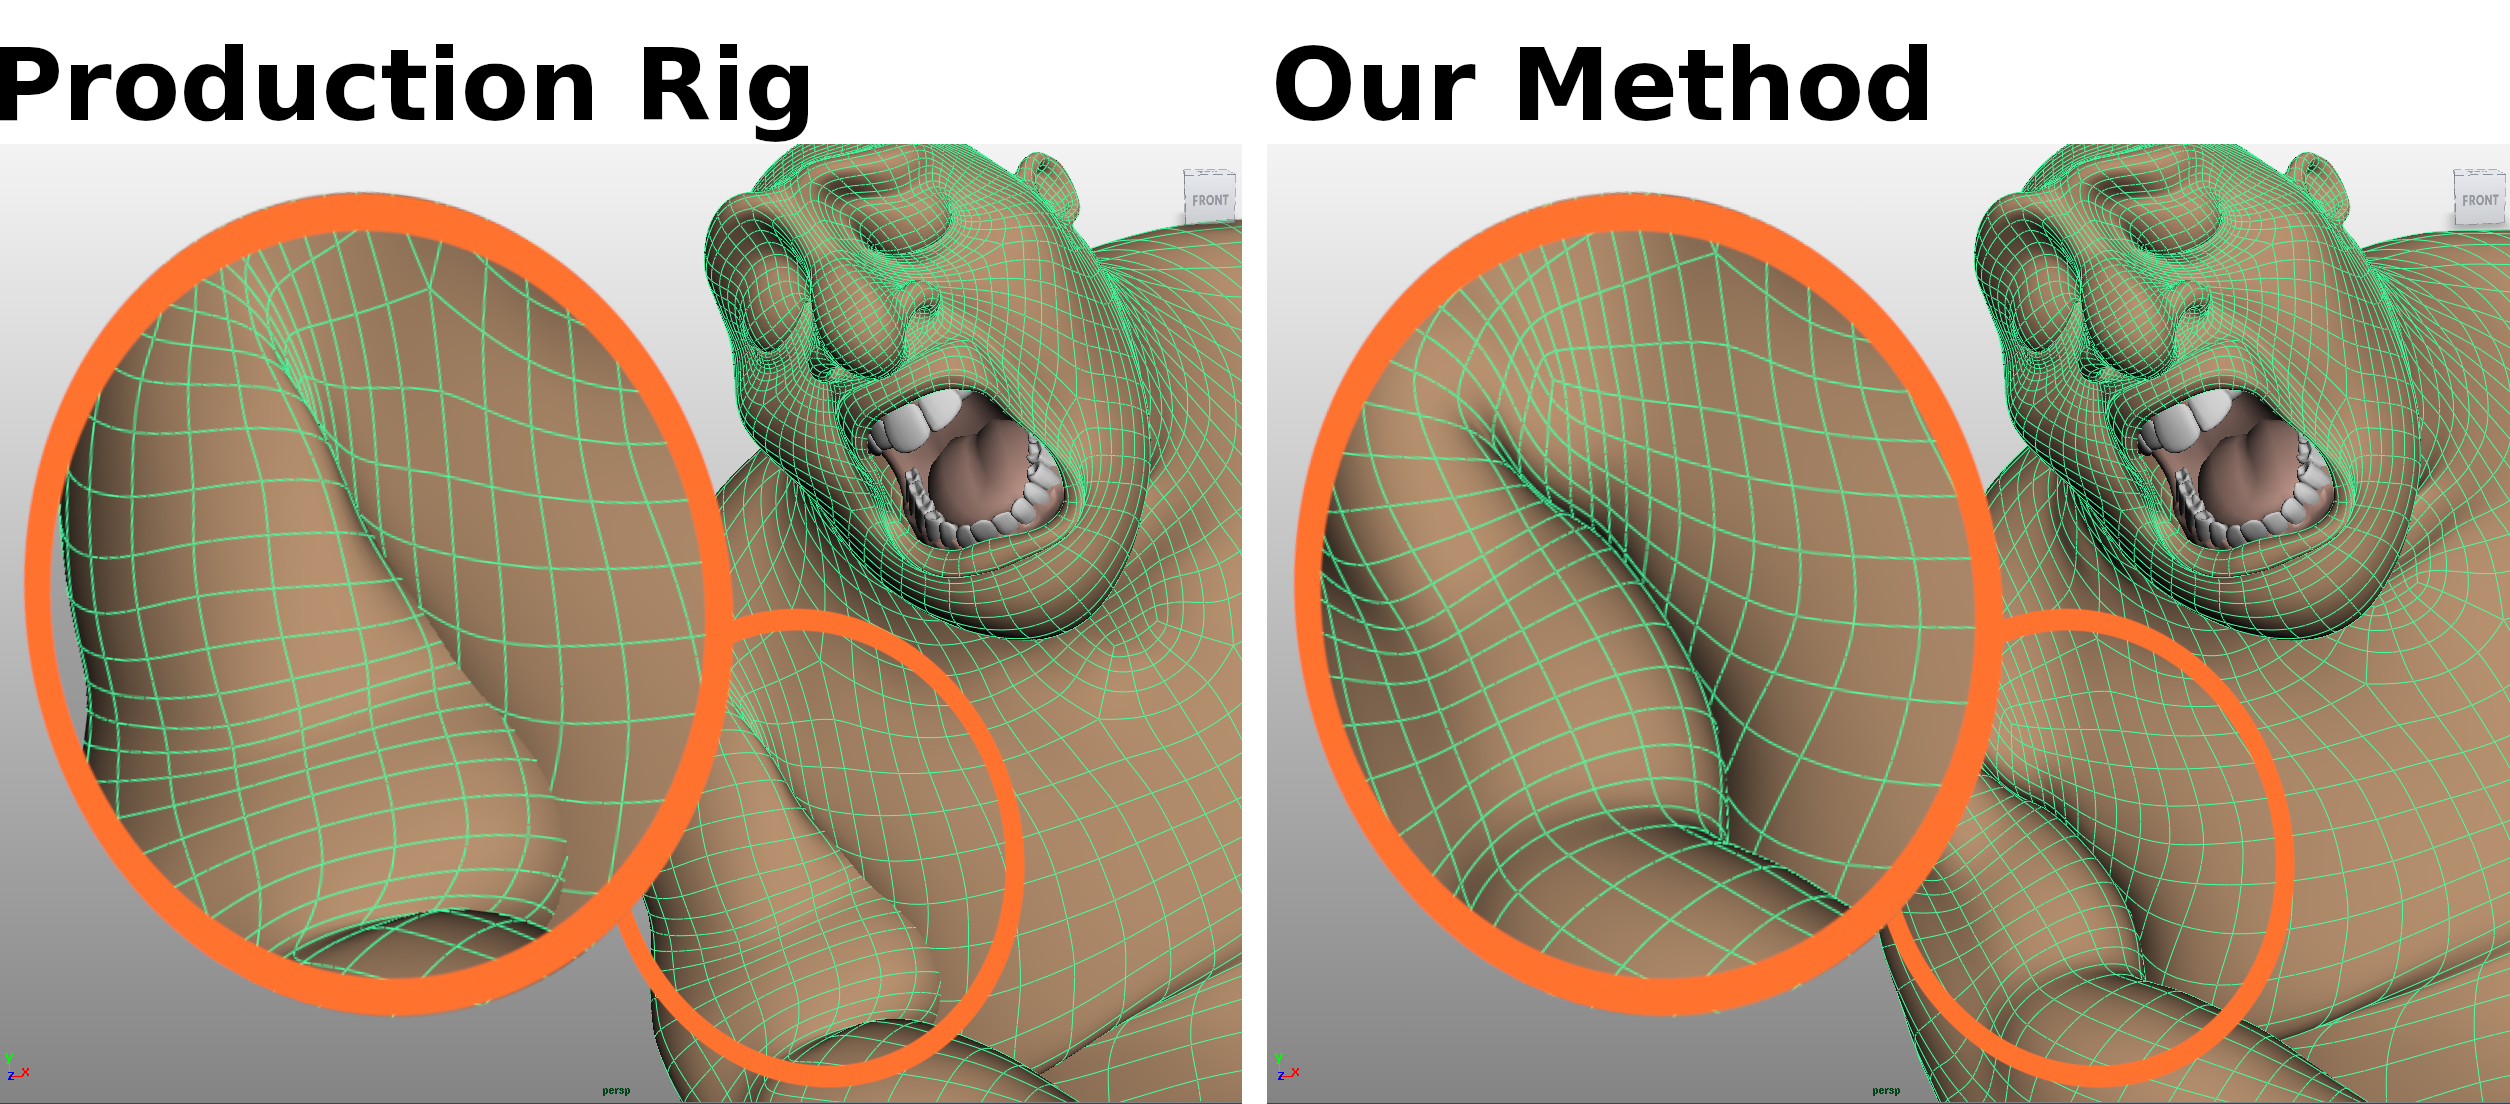
\includegraphics[width=\linewidth]{elasticity/figures/collision-figure}
\end{center}
\caption[Collisions improve deformation quality.]{Collisions and especially self-collisions drastically improve the
  quality of deformation when coupled with elasticity. On the left is a
  production rig that qualitatively exhibits the right look but does not resolve
  collisions. On the right is our method which resolves self-collisions
  producing a much more natural look.}
\label{fig:collisions}
\end{figure}

As previously discussed, the ability to handle elaborate collision is an essential benefit of simulation in production. We use point constraints to enforce both soft constraints, such as bone attachments, and to handle object and self collisions. Specifically, we embed proxy points ($\mathbf{x}_p$) in the simulation lattices and distribute their associated forces trilinearly to the vertices of the hexahedral cells that contain them. \cite{sifakis:2007:hybridsolids} show the effectiveness of this basic approach.

\paragraph{Soft constraints }
Springs attached to embedded proxy points are used to enforce soft constraints such as bone bindings. The forces from these springs are derived from the standard quadratic energy density
$\Psi(\mathbf{x}) = k/2\|\mathbf{x}-\mathbf{x}_p\|^2$.

\paragraph{Collision detection }
The collision response is determined by a number of collision proxies approximately covering the embedded collision surface. We utilize a penalty based response dependent on the penetration depth and unit outward normal at each proxy point. For rigid objects, we simply query a level set representation of the object at each proxy point. However, for self-collision, the rapidly changing shape of the elastic objects precludes accurate reconstruction of a signed distance function at each time step.

\paragraph{Self-collision penetration depth evaluation }
For each proxy collision point, we first determine which deformed hexahedra contain it in the current configuration. This is done rapidly by querying an axis aligned bounding box hierarchy whose leaves surround each deformed hexahedron in the current configuration. To prevent false positives, we do not look in the 27 hexahedra in the one ring of the proxy point in material coordinates. Each hexahedron deemed near a given proxy point is then tetrahedralized to barycentrically determine the proxy point's material location. For each material point, we query a level set stored in the undeformed configuration: $\phi_0$.  If there are multiple negative $\phi_0$ values, we use the location with $\phi_0$ closest to zero to compute the closest point on the undeformed surface. We then look up the deformed position of the closest surface point ($\mathbf{x}_s$)  to estimate the penetration depth as $\left|\mathbf{x}_s-\mathbf{x}_p\right|$ and outward unit normal as $\mathbf{n}=\left(\mathbf{x}_s-\mathbf{x}_p\right)/\left|\mathbf{x}_s-\mathbf{x}_p\right|$.

\paragraph{Collision response }
For both self-collision and solid object collision scenarios, we instantiate a zero rest-length spring from the proxy point to the closest point on the surface. The Young's modulus of this spring is allowed to be anisotropic in the direction of the unit collision normal. Specifically, the spring force arises from the energy density
$\Psi(\mathbf{x}_p,\mathbf{x}_s)=k(\mathbf{x}_p-\mathbf{x}_s)^T\mathbf{M}(\mathbf{x}_p-\mathbf{x}_s)/2$
where  $\mathbf{M}=\left(1-\alpha\right)\mathbf{n}\mathbf{n}^T+\alpha\mathbf{I}$, with $\alpha\in[0,1]$.  $\alpha=1$ corresponds with a traditional isotropic spring; $\alpha=0$ results in a standard point repulsion.  This anisotropic conception of the stiffness allows for sliding in the plane orthogonal to the penetration direction. In practice we found $\alpha\in[.1,.5]$ worked best for self collisions and $\alpha = 0$ was sufficient for object collisions.
